\subsubsection{Bothan}

\begin{samepage}
	\begin{flushright}
		\begin{tabular}{ l l }
			\textbf{Type} 			& Félin \\
		   	\textbf{Planète} 		& Bothawui \\
		   	\textbf{Language} 		& Bothese \\
		   	\textbf{Orientation} 	& Lumineux \\
		\end{tabular}
	\end{flushright}

	\vspace{-5\baselineskip}
	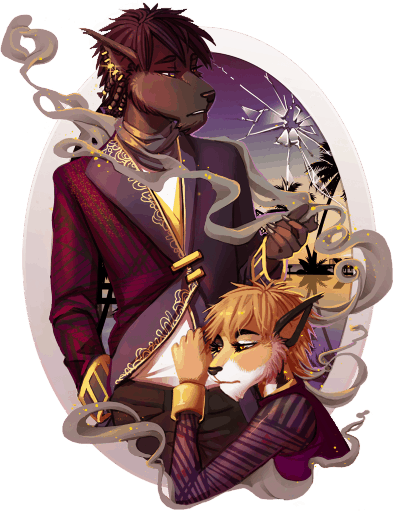
\includegraphics[width=5cm]{img/races/bothan.png}
\end{samepage}

Les Bothans sont des humanoïdes trappus, dont le corps est recouvert d'une épaisse fourrure pouvant varier du blanc-cassé à brun très foncé.
Le peuple bothan est originaire de la planète Bothawui, un monde cosmopolite épargné des troubles de la Guerre Civile Galactique en raison de la neutralité officielle du gouvernement bothan. Plusieurs colonies ont également été construites sur des planètes proches, telles que Kothlis, qui est désormais le siège d'une importante communauté. Toutes ces colonies forment l'Espace Bothan.\\
La structure sociale des Bothans est constituée par des clans familiaux, dont le nom est inclus dans le nom de chaque Bothan, à la suite d'une apostrophe.

\begin{description}[align=left]
\item [Agilité du Félin] 			% CAP +2
		Les Bothans possède la grace de leur ancêtres félins.\\
		\emph{Commence avec d6 Agi}
\item [Service de renseignement] 	% CAP +1
		Depuis plus de 300 ans ces êtres intelligents et rusés ont perfectionné leurs façons de faire, et ont développé un vaste réseau d'espions et d'informateurs destiné à recueillir toutes sortes d'informations sur les sujets les plus importants.\\
		\emph{d6 en Réseaux}
\item [Comme en plein jour] 		% CAP +1
		Grace à leur yeux de félins, les Bothans voient parfaitemnet dans l'obscurité.\\
		\emph{Vision Nocture}
\item [Déplacement rapide] 			% CAP +2
		Les Bothans, s'ils se baissent sur leur quatres pattes peuvent atteindre des vitesses de 80km/h.\\
		\emph{All = 10}
\item [Frêle] 						% CAP -2
		De contitution moins résistante, les Bothans sont moins adapté aux combats rapproché.\\
		\emph{-1 Résistance}
\item [Mauvaise réputation] 		% CAP -1
		Les ruses conduites par ce peuple, ainsi que l'opacité inhérente au Réseau Bothan, ne jouent pas en leur faveur. Certains leur reprochent de ne pas avoir prévu que l'Empire tendait une embuscade aux forces de l'Alliance.\\
		\emph{\'Etranger}
\item [Prudent] 					% CAP -1
		Les Bothans ne font rien à la légère, ils ne laissent nulle place au hazard et chaque décision est murrement réfléchie. Ils ne connaissent pas l'urgence.\\
		\emph{Prudent}
\end{description}